\documentclass{article}
\usepackage{tikz}
\usetikzlibrary{automata,positioning}

\begin{document}

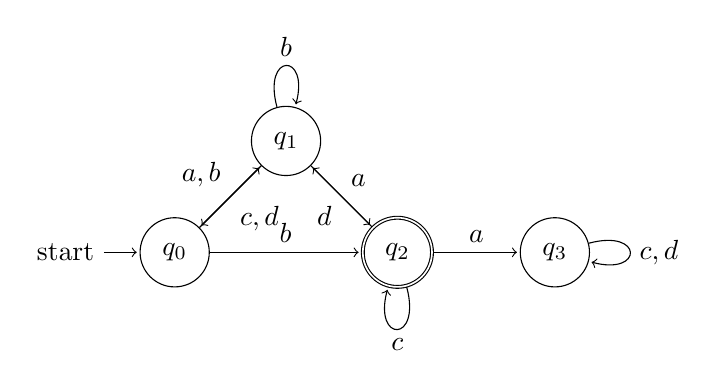
\begin{tikzpicture}[shorten >=1pt,node distance=2cm,on grid,auto]
    \node[state,initial] (q_0) {$q_0$};
    \node[state] (q_1) [above right=of q_0] {$q_1$};
    \node[state,accepting] (q_2) [below right=of q_1] {$q_2$};
    \node[state] (q_3) [right=of q_2] {$q_3$};

    \path[->]
    (q_0) edge node {$a,b$} (q_1)
          edge node {$b$} (q_2)
    (q_1) edge [loop above] node {$b$} ()
          edge node {$c,d$} (q_0)
          edge node {$a$} (q_2)
    (q_2) edge [loop below] node {$c$} ()
          edge node {$a$} (q_3)
          edge node {$d$} (q_1)
    (q_3) edge [loop right] node {$c,d$} ();
\end{tikzpicture}

\end{document}